% Szglab4
% ===========================================================================
%
\chapter{Grafikus felület specifikációja}

\thispagestyle{fancy}

\section{A grafikus interfész}
%\comment{A menürendszer, a kezelői felület grafikus képe. A grafikus felület megjelenését, a használt ikonokat, stb screenshot-szerű képekkel kell bemutatni. Az építészetben ez a homlokzati terv.}
A szoftvert elindítva megjelenik egy grafikus ablak a következő tartalommal:

\begin{figure}[H]
\begin{center}
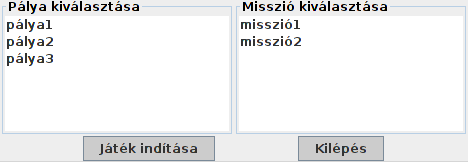
\includegraphics[width=10cm]{images/ch11/screenshot_menu.png}
\caption{A menü kinézete}
\label{fig:screenshot_menu}
\end{center}
\end{figure}

Értelemszerűen a bal oldali listában az elérhető pályák közül választhatja ki a felhasználó azt, amelyiken játszani szeretne, a jobb oldaliban pedig a kiválasztott pályához tartozó missziók közül azt, amelyiket el kívánja indítani.

Az alul látható gombok közül a "Kilépés" feliratú bezárja az alkalmazást, a "Játék indítása" feliratú pedig a fent kijelölt paraméterekkel elindítja a játékot. Ekkor az ablak átméreteződik, tartalma kicserélődik erre:

\begin{figure}[H]
\begin{center}
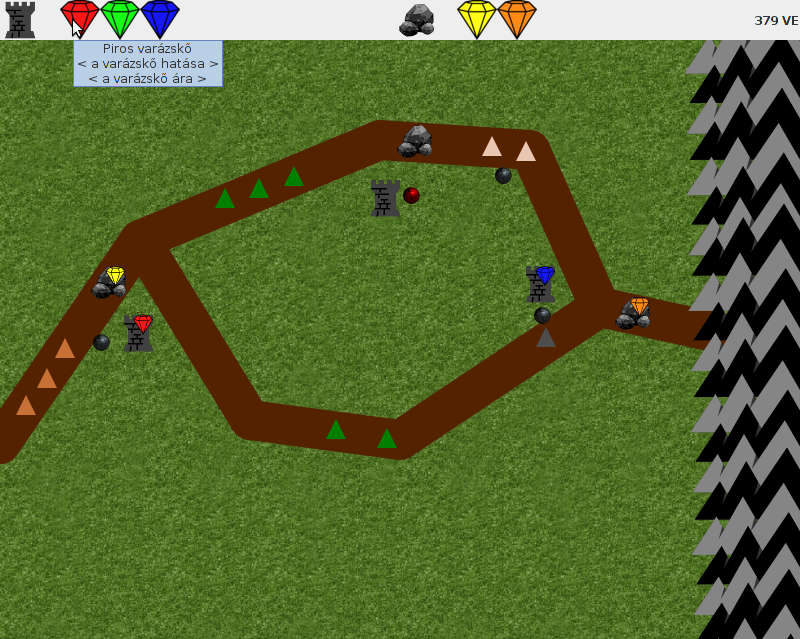
\includegraphics[width=14cm]{images/ch11/screenshot_game.png}
\caption{A játék képe}
\label{fig:screenshot_game}
\end{center}
\end{figure}

Az ablak felső részében a menüsáv, alatta pedig a játéktér foglal helyet.

A menüsávban lévő kis ikonok segítségével a következő funkciók érhetők el (balról jobbra haladva):

\begin{itemize}
\item Torony ikon: Először erre, majd a játéktéren egy megfelelő helyre (nem útra) kattintva egy torony építhető
\item Piros, zöld és kék varázskő ikonok: Először ezekre, majd a játéktéren egy toronyra kattintva egy torony erősíthető a kiválasztott varázskővel
\item Akadály ikon: Először erre, majd a játéktéren egy megfelelő helyre (útra) kattintva egy akadály építhető
\item Sárga és narancssárga varázskő ikonok: Először ezekre, majd a játéktéren egy akadályra kattintva egy akadály erősíthető a kiválasztott varázskővel
\end{itemize}

A menüsáv jobb szélén pedig a jelenleg rendelkezésre álló varázserőnket olvashatjuk le.\\
\\
Ahogyan a fenti ábrán is látszik, az egérmutatót a varázskő ikonokon tartva egy felugró eszköztipp ablakban megjelenik néhány sor szöveg, amely leírja a kiválasztott varázskő nevét, tulajdonságait, és varázserőben mért árát.\\
\\
A játéktér jeleníti meg a csata pillanatnyi állapotát. A barna vonalak az ellenség útvonalai, amelyeken az ablak jobb szélen látható Végzet Hegye felé tartanak.\\
\\
Az egyes ellenségeket különbözű színű háromszögek szimbolizálják. A sötétebb narancssárga embert, a halványrózsaszín hobbitot, a zöld tündét, a szürke pedig törpöt jelent.\\
\\
A tornyok magától értetődő ábrával jelennek meg, az akadályok az utakon pedig egy három szikladarabot ábrázoló kép formájában.\\
\\
Azon tornyok és akadályok képe fölött, amelyek már meg lettek erősítve varázskővel, a rajtuk lévő kő ikonja megjelenik a jobb felső sarokban.\\
\\
A tornyok által az ellenségekre kilőtt lövedékek a fekete, míg a különleges, kettévágó lövedékek a piros golyók.\\
\\
Az alkalmanként leszálló köd az egész játékteret beborító halvány, szürkés átfedés formájában fog megjelenni.\\
\\
Összefoglaló áttekintés a játéktér ikonjairól (nem méretarányosan):

\begin{figure}[ht]
\centering

\subfigure[Torony]{

\includegraphics[width=2cm]{images/ch11/icons/tower.png}
    \label{overview:tower}
}
\subfigure[Akadály]{

\includegraphics[width=2cm]{images/ch11/icons/obstacle.png}
    \label{overview:obstacle}
}
\subfigure[Varázskő]{

\includegraphics[width=2cm]{images/ch11/icons/blue_gem.png}
    \label{overview:gem}
}
\subfigure[Ellenség]{

\includegraphics[width=2cm]{images/ch11/icons/human.png}
    \label{overview:enemy}
}
\subfigure[Lövedék]{

\includegraphics[width=2cm]{images/ch11/icons/projectile.png}
    \label{overview:projectile}
}
\subfigure[Kettévágó lövedék]{

\includegraphics[width=2cm]{images/ch11/icons/splitter_projectile.png}
    \label{overview:splitter_projectile}
}
\caption{Áttekintés az ikonokról}
\label{fig:icon_overview}
\end{figure}

\newpage

\section{A grafikus rendszer architektúrája}
%\comment{A felület működésének elve, a grafikus rendszer architektúrája (struktúra diagramok). A struktúra diagramokon a prototípus azon és csak azon osztályainak is szerepelnie kell, amelyekhez a grafikus felületet létrehozó osztályok kapcsolódnak.}

\subsection{A felület működési elve}
A grafikus felületet MVC architektúrának megfelelően próbáltuk megtervezni. Minden képernyőn megjelenő objektumnak van egy grafikus párja, ami megvalósítja a \textbf{Drawable} interfészt. A \textbf{View} osztály ilyen objektumokat tárol, és minden kirajzolásnál meghívja ezen objektumok draw metódusát. \\
A megjelenítés push alapú. Ha a modelben történt valami változás (amit hívhatunk egy eseménynek), akkor értesíti a \textbf{View}-t, hogy valami esemény történt, úgy hogy meghívja az eseménynek megfelelő metódust. Kirajzolásnál minden grafikus objektum, lekérdezi a \textbf{Game}-ben lévő párjától az adatait, majd ez alapján kirajzolja magát.\\
Az MVC megvalósítás alól kivételt képez a program indulása, amikor is egy egyszerű menü jelenik, amin el lehet indítani a játékot, ezt a \textbf{Menu} osztály végzi.\\
A \textbf{Controller} osztály a program elején, a \textbf{Game} és \textbf{View} objektumok létrehozása után feliratkozik a neki megfelelő eseményekre. Ez után már fogadja is az eseményeket.\\
Tervezés során ügyletünk arra is, hogy könnyen bővíthető, cserélhető legyen a rendszer. A \textbf{View} és \textbf{Graphic} osztályokból való származtatással új GUI-t lehet készíteni, anélkül, hogy meglévő kódban kelljen (sokat) változtatni.

\subsection{A felület osztály-struktúrája}
%\comment{Osztálydiagram. Minden új osztály, és azon régiek, akik az újakhoz közvetlenül kapcsolódnak.}

\begin{figure}[H]
\begin{center}
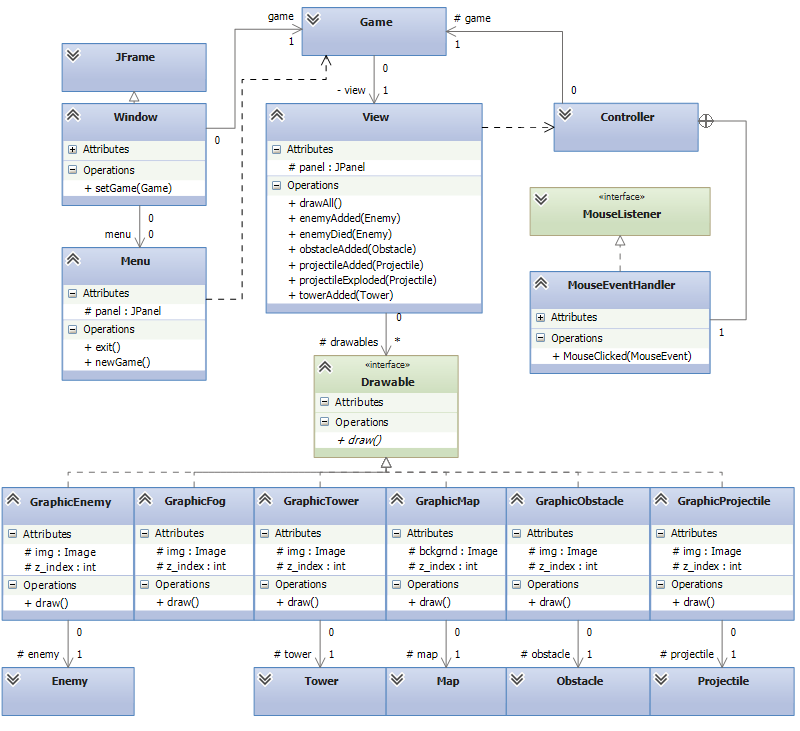
\includegraphics[width=18cm]{images/ch11/very_uml_class_tiny.png}
\caption{Grafikus felület osztálydigaramja}
\label{fig:Graphic_class_diag}
\end{center}
\end{figure}

\section{A grafikus objektumok felsorolása}
\comment{Az új osztályok felsorolása. Az régi osztályok közül azoknak a felsorolása, ahol változás volt. Ezek esetén csak a változásokat kell leírni.}

\subsection{Osztály1}
\begin{itemize}
\item Felelősség\newline
\comment{Mi az osztály felelőssége. Kb 1 bekezdés. Ha szükséges, akkor state-chart is.}
\item Ősosztályok\newline
\comment{Mely osztályokból származik (öröklési hierarchia)\newline
Legősebb osztály $\rightarrow$ Ősosztály2 $\rightarrow$ Ősosztály3...}
\item Interfészek\newline
\comment{Mely interfészeket valósítja meg.}
\item Attribútumok\newline
\comment{Milyen attribútumai vannak}
	\begin{itemize}
		\item attribútum1: attribútum jellemzése: mire való, láthatósága (UML jelöléssel), típusa
		\item attribútum2: attribútum jellemzése: mire való, láthatósága (UML jelöléssel), típusa
	\end{itemize}
\item Metódusok\newline
\comment{Milyen publikus, protected és privát  metódusokkal rendelkezik. Metódusonként precíz leírás, ha szükséges, activity diagram is  a metódusban megvalósítandó algoritmusról.}
	\begin{itemize}
		\item int foo(Osztály3 o1, Osztály4 o2): metódus leírása, láthatósága (UML jelöléssel)
		\item int bar(Osztály5 o1): metódus leírása, láthatósága (UML jelöléssel)
	\end{itemize}
\end{itemize}

\subsection{Osztály2}
\begin{itemize}
\item Felelősség\newline
\comment{Mi az osztály felelőssége. Kb 1 bekezdés. Ha szükséges, akkor state-chart is.}
\item Ősosztályok\newline
\comment{Mely osztályokból származik (öröklési hierarchia)\newline
Legősebb osztály $\rightarrow$ Ősosztály2 $\rightarrow$ Ősosztály3...}
\item Interfészek\newline
\comment{Mely interfészeket valósítja meg.}
\item Attribútumok\newline
\comment{Milyen attribútumai vannak}
	\begin{itemize}
		\item attribútum1: attribútum jellemzése: mire való, láthatósága (UML jelöléssel), típusa
		\item attribútum2: attribútum jellemzése: mire való, láthatósága (UML jelöléssel), típusa
	\end{itemize}
\item Metódusok\newline
\comment{Milyen publikus, protected és privát  metódusokkal rendelkezik. Metódusonként precíz leírás, ha szükséges, activity diagram is  a metódusban megvalósítandó algoritmusról.}
	\begin{itemize}
		\item int foo(Osztály3 o1, Osztály4 o2): metódus leírása, láthatósága (UML jelöléssel)
		\item int bar(Osztály5 o1): metódus leírása, láthatósága (UML jelöléssel)
	\end{itemize}
\end{itemize}

\section{Kapcsolat az alkalmazói rendszerrel}
\comment{Szekvencia-diagramokon ábrázolni kell a grafikus rendszer működését. Konzisztens kell legyen az előző alfejezetekkel. Minden metódus, ami ott szerepel, fel kell tűnjön valamelyik szekvenciában. Minden metódusnak, ami szekvenciában szerepel, szereplnie kell a valamelyik osztálydiagramon.}

